\documentclass[12pt,letterpaper]{article}
\usepackage{graphicx,textcomp}
\usepackage{natbib}
\usepackage{setspace}
\usepackage{fullpage}
\usepackage{color}
\usepackage[reqno]{amsmath}
\usepackage{amsthm}
\usepackage{fancyvrb}
\usepackage{amssymb,enumerate}
\usepackage[all]{xy}
\usepackage{endnotes}
\usepackage{lscape}
\newtheorem{com}{Comment}
\usepackage{float}
\usepackage{hyperref}
\newtheorem{lem} {Lemma}
\newtheorem{prop}{Proposition}
\newtheorem{thm}{Theorem}
\newtheorem{defn}{Definition}
\newtheorem{cor}{Corollary}
\newtheorem{obs}{Observation}
\usepackage[compact]{titlesec}
\usepackage{dcolumn}
\usepackage{tikz}
\usetikzlibrary{arrows}
\usepackage{multirow}
\usepackage{xcolor}
\newcolumntype{.}{D{.}{.}{-1}}
\newcolumntype{d}[1]{D{.}{.}{#1}}
\definecolor{light-gray}{gray}{0.65}
\usepackage{url}
\usepackage{listings}
\usepackage{color}

\definecolor{codegreen}{rgb}{0,0.6,0}
\definecolor{codegray}{rgb}{0.5,0.5,0.5}
\definecolor{codepurple}{rgb}{0.58,0,0.82}
\definecolor{backcolour}{rgb}{0.95,0.95,0.92}

\lstdefinestyle{mystyle}{
	backgroundcolor=\color{backcolour},   
	commentstyle=\color{codegreen},
	keywordstyle=\color{magenta},
	numberstyle=\tiny\color{codegray},
	stringstyle=\color{codepurple},
	basicstyle=\footnotesize,
	breakatwhitespace=false,         
	breaklines=true,                 
	captionpos=b,                    
	keepspaces=true,                 
	numbers=left,                    
	numbersep=5pt,                  
	showspaces=false,                
	showstringspaces=false,
	showtabs=false,                  
	tabsize=2
}
\lstset{style=mystyle}
\newcommand{\Sref}[1]{Section~\ref{#1}}
\newtheorem{hyp}{Hypothesis}

\title{Problem Set 2}
\date{Vanessa Wong}
\author{QTM 200: Applied Regression Analysis}

\begin{document}
	\maketitle
	
	\section*{Instructions}
	\begin{itemize}
		\item Please show your work! You may lose points by simply writing in the answer. If the problem requires you to execute commands in \texttt{R}, please include the code you used to get your answers. Please also include the \texttt{.R} file that contains your code. If you are not sure if work needs to be shown for a particular problem, please ask.
		\item Your homework should be submitted electronically on the course GitHub page in \texttt{.pdf} form.
		\item This problem set is due at the beginning of class on Monday, February 10, 2020. No late assignments will be accepted.
		\item Total available points for this homework is 100.
	\end{itemize}
	
	\vspace{.5cm}
	\section*{Question 1 (40 points): Political Science}
		\vspace{.25cm}
	The following table was created using the data from a study run in a major Latin American city.\footnote{Fried, Lagunes, and Venkataramani (2010). ``Corruption and Inequality at the Crossroad: A Multimethod Study of Bribery and Discrimination in Latin America. \textit{Latin American Research Review}. 45 (1): 76-97.} As part of the experimental treatment in the study, one employee of the research team was chosen to make illegal left turns across traffic to draw the attention of the police officers on shift. Two employee drivers were upper class, two were lower class drivers, and the identity of the driver was randomly assigned per encounter. The researchers were interested in whether officers were more or less likely to solicit a bribe from drivers depending on their class (officers use phrases like, ``We can solve this the easy way'' to draw a bribe). The table below shows the resulting data.

\begin{table}[h!]
	\centering
	\begin{tabular}{l | c c c }
		& Not Stopped & Bribe requested & Stopped/given warning \\
		\\[-1.8ex] 
		\hline \\[-1.8ex]
		Upper class & 14 & 6 & 7 \\
		Lower class & 7 & 7 & 1 \\
		\hline
	\end{tabular}
\end{table}

\begin{itemize}
	
	\item [(a)]
	Calculate the $\chi^2$ test statistic by hand (even better if you can do "by hand" in \texttt{R}).\\
	\vspace{1cm}
	\item
		The chi-squared test statistic is 3.791168.
	\lstinputlisting[language=R, firstline=40, lastline=61]{PS2_answers.R}
	\vspace{1cm}
	\item [(b)]	Now calculate the p-value (in \texttt{R}).\footnote{Remember frequency should be $>$ 5 for all cells, but let's calculate the p-value here anyway.}  What do you conclude if $\alpha = .1$?\\
	\item
		p-value = 0.1502 \textgreater 0.1, therefore we conclude that there is not enough evidence to reject (i.e. fail to reject) the null hypothesis that x and y are statistically independent.
		\lstinputlisting[language=R, firstline=66, lastline=69]{PS2_answers.R}
		\newpage
	\item [(c)] Calculate the standardized residuals for each cell and put them in the table below.
	\vspace{1cm}
	\begin{table}[h]
		\centering
		\begin{tabular}{l | c c c }
			& Not Stopped & Bribe requested & Stopped/given warning \\
			\\[-1.8ex] 
			\hline \\[-1.8ex]
			Upper class  &0.322  &-1.642  &1.523  \\ 
			\\ 
			Lower class &-0.322  &1.642   &-1.523  \\
		
		\end{tabular}
	\end{table}
	\lstinputlisting[language=R, firstline=71, lastline=87]{PS2_answers.R}
	
	\vspace{2cm}
	\item [(d)] How might the standardized residuals help you interpret the results?  
	\item
	Standardized residuals show how much each cell's observed value deviates from its respective expected value, which is the value that would be obtained if X and Y were independent variables.
	
\end{itemize}


\section*{Question 2 (20 points): Economics}
Chattopadhyay and Duflo were interested in whether women promote different policies than men.\footnote{Chattopadhyay and Duflo. (2004). ``Women as Policy Makers: Evidence from a Randomized Policy Experiment in India. \textit{Econometrica}. 72 (5), 1409-1443.} Answering this question with observational data is pretty difficult due to potential confounding problems (e.g. the districts that choose female politicians are likely to systematically differ in other aspects too). Hence, they exploit a randomized policy experiment in India, where since the mid-1990s, $\frac{1}{3}$ of village council heads have been randomly reserved for women. A subset of the data from West Bengal can be found at the following link: \url{https://raw.githubusercontent.com/kosukeimai/qss/master/PREDICTION/women.csv}\\

\noindent Each observation in the data set represents a village and there are two villages associated with one GP (i.e. a level of government is called "GP"). Figure~\ref{fig:women_desc} below shows the names and descriptions of the variables in the dataset. The authors hypothesize that female politicians are more likely to support policies female voters want. Researchers found that more women complain about the quality of drinking water than men. You need to estimate the effect of the reservation policy on the number of new or repaired drinking water facilities in the villages.
\vspace{.5cm}
\begin{figure}[h!]
	\caption{\footnotesize{Names and description of variables from Chattopadhyay and Duflo (2004).}}
	\vspace{.5cm}
	\centering
	\label{fig:women_desc}
	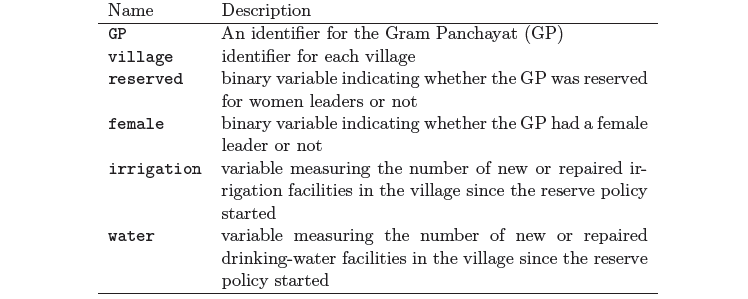
\includegraphics[width=1.1\textwidth]{../women_desc.png}
\end{figure}		

\begin{itemize}
	\item [(a)] State a null and alternative (two-tailed) hypothesis. 
	\item 
	Null: there is no relationship between the GP being reserved for female leaders and the {\#} new/repaired drinking water facilities is 0
	\item
	Alternative: there exists some relationship between the GP being reserved for women leaders and {\#} new/repaired drinking water facilities
	\vspace{1cm}
	\newpage
	\item [(b)] Run a bivariate regression to test this hypothesis in \texttt{R} (include your code!).
	\item
	Linear model: y = 14.378 + 9.252x
	\lstinputlisting[language=R, firstline=101, lastline=138]{PS2_answers.R}
	\vspace{2cm}
	\item [(c)] Interpret the coefficient estimate for reservation policy. 
	\item
	$\alpha = 14.738$\\. When the GP is not reserved for women leaders (i.e. reserved = 0), the predicted number of new or repaired drinking-water facilities in the village is 0.3029.
	\item
	$\beta = 9.252$\\. For each additional GP that is reserved for women leaders, the number of new or repaired drinking-water facilities increases by 9.252.
	
\end{itemize}

	\section*{Question 3 (40 points): Biology}

There is a physiological cost of reproduction for fruit flies, such that it reduces the lifespan of female fruit flies.  Is there a similar cost to male fruit flies?  This dataset contains observations from five groups of 25 male fruit flies. The experiment tests if increased reproduction reduces longevity for male fruit flies. The five groups are: males forced to live alone, males assigned to live with one or eight newly pregnant females (non-receptive females), and males assigned to live with one or eight virgin females (interested females). The name of the data set is \texttt{fruitfly.csv}.\footnote{Partridge and Farquhar (1981).``Sexual Activity and the Lifespan of Male Fruitflies''. \textit{Nature}. 294, 580-581.}
	\vspace{1cm}

\begin{tabular}{r|l}
	\texttt{No} & serial number (1-25) within each group of 25\\
	\texttt{type} & Type of experimental assignment \\
	& \hspace{0.1in} $1=$ no females  \\
	& \hspace{0.1in} $2=$ 1 newly pregnant female \\
	& \hspace{0.1in} $3=$ 8 newly pregnant females\\
	& \hspace{0.1in} $4=$ 1 virgin female\\
	& \hspace{0.1in} $5=$ 8 virgin females\\
	\texttt{lifespan} & lifespan (days)\\
	\texttt{thorax} & length of thorax (mm)\\
	\texttt{sleep} & percentage of each day spent sleeping\\
\end{tabular}
	\vspace{1cm}
\newpage
\begin{itemize} 
		\item Import the data set and obtain summary statistiscs and examine the distribution of the overall lifespan of the fruitflies.
	\item
	The distribution of overall fruitfly lifespan appears to be bimodal and approximately normal (there is a slight left skew -- median is greater than the mean).
	\begin{itemize}
		\item 
		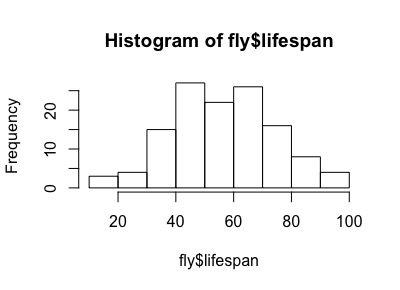
\includegraphics{Histogramlifespan.jpeg}
	\end{itemize}
	\item Summary statistics for fruitfly lifespan:
	\begin{tabular}{r|l}
		\texttt{Min} & 16\\
		\texttt{Q1} & 46 \\
		\texttt{Median} & 58 \\
		\texttt{Mean} & 57.44 \\
		\texttt{Q3} & 70 \\
		\texttt{Max} & 97 \\
\end{tabular}
\lstinputlisting[language=R, firstline=150, lastline=156]{PS2_answers.R}
	\item
	Plot \texttt{lifespan} vs \texttt{thorax}. Does it look like there is a linear relationship? Provide the plot. What is the correlation coefficient between these two variables?
		\vspace{0.5cm}
\begin{itemize}
	\item
	There appears to be a linear relationship between fruitfly thorax and lifespan length. r= 0.636. There is a moderate positive correlation between fruitfly thorax length and fruitfly lifespan.
	\begin{itemize}
		\item 
	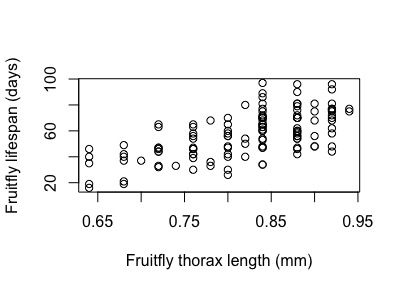
\includegraphics{lifespanvsthorax}
\end{itemize}
	\lstinputlisting[language=R, firstline=159, lastline=166]{PS2_answers.R}
	
\end{itemize}
		\vspace{1 cm}
	\item
	Regress \texttt{lifespan} on \texttt{thorax}.  Interpret the slope of the fitted model.
			\vspace{0.5cm}
\begin{itemize}
	\item
	Interpretation of beta/slope: For every one mm increase in fruitfly thorax length, there is a 144.33 day increase in fruitfly lifespan.
	\item
	Linear model: y = -61.05 + 144.33x
		\lstinputlisting[language=R, firstline=168, lastline=190]{PS2_answers.R}
\end{itemize}
\vspace{1cm}
	\item
	Test for a significant linear relationship between  \texttt{lifespan} and \texttt{thorax}. Provide and interpret your results of your test.
\begin{itemize}
	\item
	p ~ 0 , therefore there is a statistically reliable and significant linear relationship between fruitfly thorax and lifespan length.
\end{itemize}
	\lstinputlisting[language=R, firstline=192, lastline=198]{PS2_answers.R}
	\item
	
	Provide the 90\% confidence interval for the slope of the fitted model.
	
			\vspace{.5cm}
	\begin{itemize}
		\item
		Use the formula for typical confidence intervals to find the 90\% confidence interval around the point estimate.		\vspace{.5cm}
		\item
		Now, try using the function  \texttt{confint()}  in \texttt{R}.
		\item
		90\% confidence interval for the slope of the fitted model is (118.3915, 170.2748). 0 is not within the interval, supporting the conclusion from the previous quesiton that there is a statistically reliable relationship between fruitfly lifespan and thorax length.
	\end{itemize}
	\lstinputlisting[language=R, firstline=201, lastline=219]{PS2_answers.R}
			\vspace{1cm}
	\item Use the \texttt{predict()} function in \texttt{R} to (1) predict an individual fruitfly's lifespan when \texttt{thorax}=0.8 and (2) the average \texttt{lifespan} of fruitflies when \texttt{thorax}=0.8 by the fitted model. This requires that you compute prediction and confidence intervals. What are the expected values of lifespan? What are the prediction and confidence intervals around the expected values? 
	\begin{itemize}
	\item
	The predicted range for an individual fruitfly's lifespan when thorax length = 0.8 is 27.375 to 81.454 days. The point estimate/expected value is 54.414 days.
	\item
	The predicted range for the average lifepsan of fruitflies when thorax length = 0.8 is 51.919 to 56.910 days. The point estimate/expected value is 54.414 days.
	\end{itemize}
	\lstinputlisting[language=R, firstline=221, lastline=228]{PS2_answers.R}
			\vspace{0.5cm}
	\item	For a sequence of \texttt{thorax} values, draw a plot with their fitted values for \texttt{lifespan}, as well as the prediction intervals and confidence intervals.
	\begin{itemize}
		\item 
	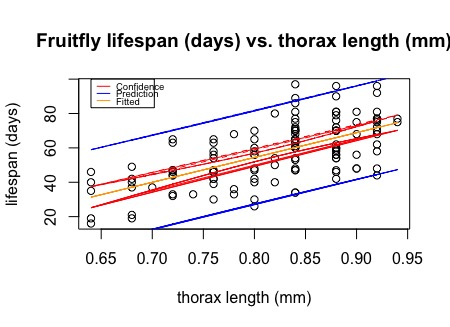
\includegraphics{confpredicplot2}
	\end{itemize}
	\lstinputlisting[language=R, firstline=233, lastline=244]{PS2_answers.R}

\end{itemize}
\begin{itemize}
	\item  R Code:
\lstinputlisting{PS2_answers.R}
\end{itemize}
\end{document}
